%!TEX root=./report.tex
\section{Appendix}
\begin{figure}[h!]
	\centering
	\includegraphics[width=0.49\linewidth]{cifar10}
	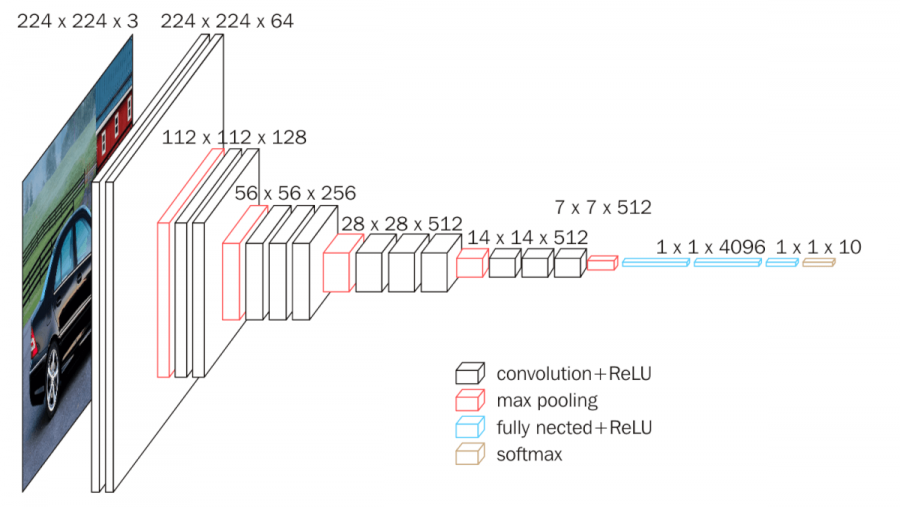
\includegraphics[width=0.49\linewidth]{vgg16}
	\caption{Left: A subset of the CIFAR-10 small image data set with ten classes. Right: The used implementation of the VGG-16 network with batch normalization.}	
	\label{fig:cifar-vgg}
\end{figure}

\begin{figure}[h!]
	\centering
	\includegraphics[width=0.49\linewidth]{mnist}
	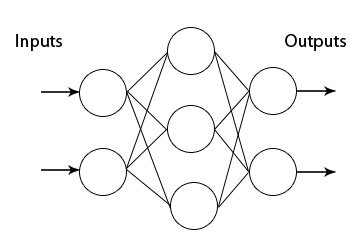
\includegraphics[width=0.49\linewidth]{two_layer_perceptron}
	\caption{Left: A subset of the MNIST handwritten digit data set. Right: An exemplary two layer perceptron with one input layer, one hidden layer of hidden unit size three and one output layer.}	
	\label{fig:mnist-two-layer}
\end{figure}